\chapter{Evaluation}
\label{chapter:evaluation}
In this chapter, we will describe our experimental evaluations, including the impact of each experiment, how we set up to examine, and to what degree our experiments help improve the performance respectively.

% spot concept drift
\section{Concept Drift Evaluation}

To avoid the model becoming gradually outdated, it is wise to update it on a timely manner. Therefore, it is essential to identify concept drift as well as keep updating the model in a strategy that is fitted to the detected concept drift.

\subsection{Evaluating the Impact of the Horizon after convergence}
To analyze the impact of keeping more or less outdated information, we let our model train on older windows and be tested on newer windows, and we let the number of windows in-between (the horizon) vary. (Note that this corresponds to giving more or less episodic memory to the model).

In the interest of simplicity, we keep the training on older windows constant and restricted to learning only on a batch of one window. We test on window sets further and further ahead of the old window; for now only one window each time.

Hence, in our simplified experimental setup, we train on Window 1 and test in turn on Window 2, on Window 3, etc.

We present the performance by plotting the AUC score against the index of the window tested.
Our results are illustrated in Figure~\ref{fig:AUC_onFurther_windows}.

\begin{figure}[htbp!]
	\centering
	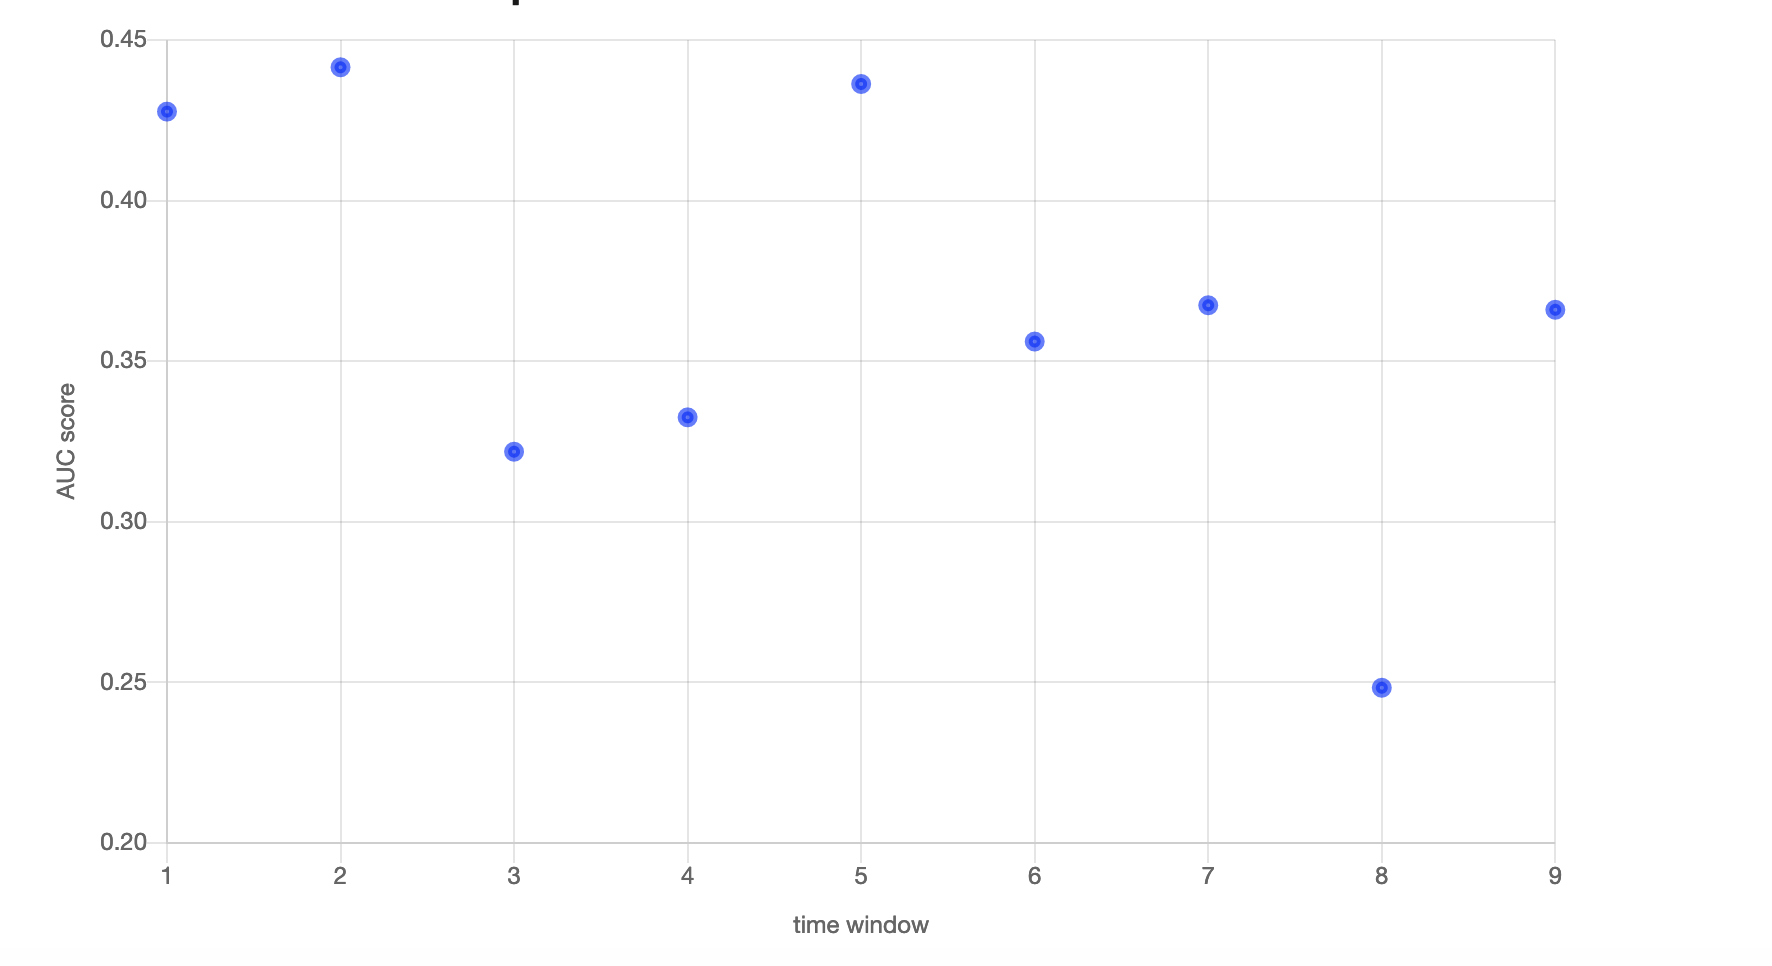
\includegraphics[width=0.6\linewidth]{images/plots/concept_drift_capture.png}
	\caption{Illustration of the impact of concept drift on the representation quality: AUC for testing windows further and further ahead from the train window.}
	\label{fig:AUC_onFurther_windows}
\end{figure}

The AUC appears to decrease as we are testing on later and later windows.

This confirms the concept drift: The dependency of the output on time changes over time, the model will not be able to capture this change, thus the trained model performs worse when the time window slides by. So, we succeed to capture concept drift. 

\subsection{Evaluating the Impact of Adaptive Incremental Learning}

% 1. Say we want to investigate sth. and why it will bring us useful insights.
We want to study the impact of incremental learning, i.e., training on recent data, on the convergence behavior, i.e., how fast the model converges and with what performance while training but, more importantly, when testing subsequently.

% 2. Say how we investigate that thing, i.e., experimental setup.
We design our experiment as follows. We compare a model that learns from earlier windows with a model that learns from recent windows, and we test each time on a window later in the sequence.
In the no incremental learning setup, at every epoch, we train the model over window 1 and 2, then test on window 20; in the full incremental learning setup, at each epoch, we train on window 18 and 19, then test again on window 20.

% 3. Say our results are presented in Material XYZ (plot/table)
We present our results in Figure~\ref{fig:comparison_concept_drift}.
% 
\begin{figure}[htbp!]
     \centering
     \begin{subfigure}[b]{0.49\textwidth}
         \centering
         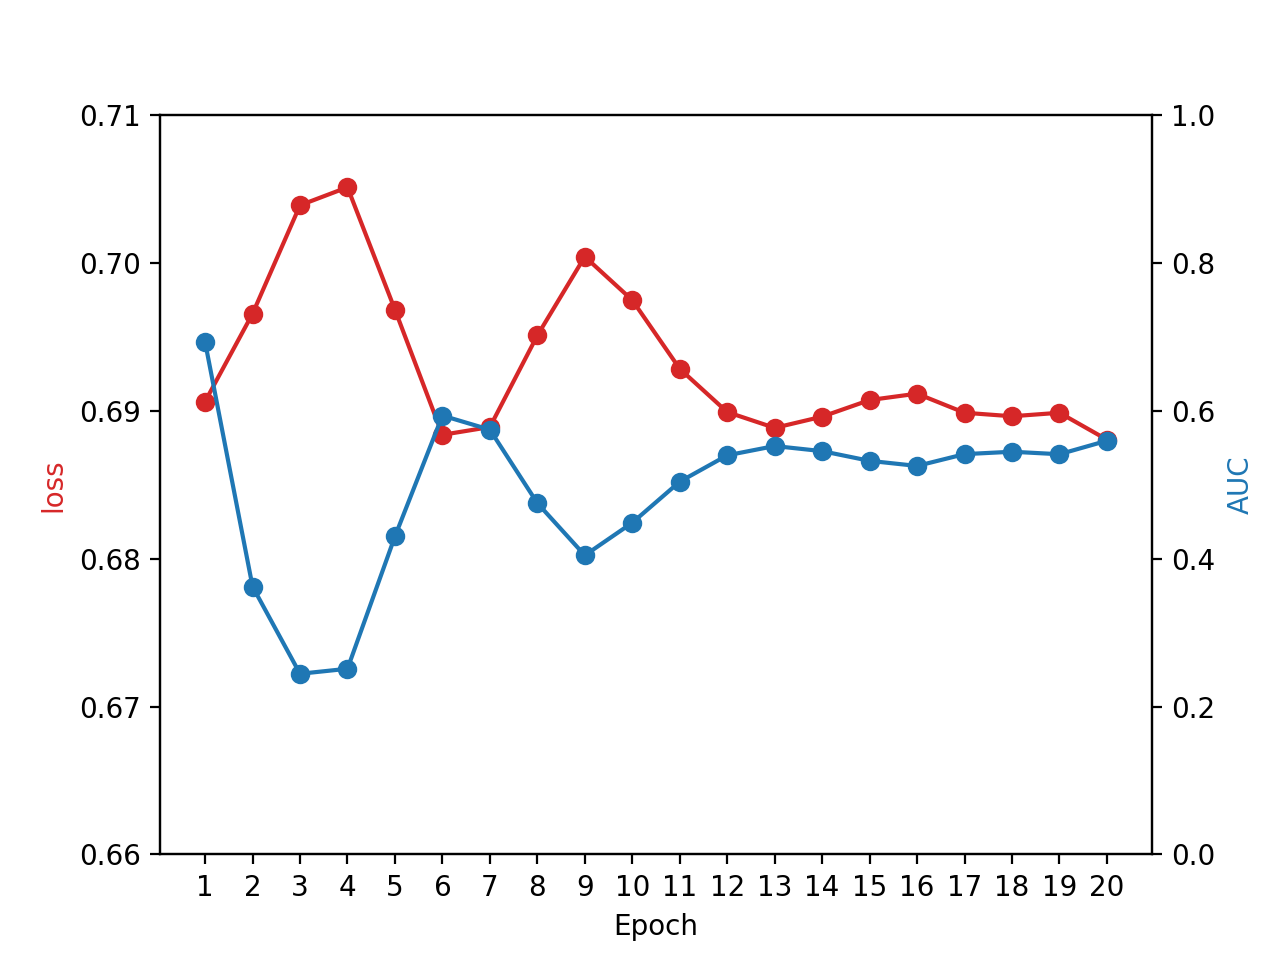
\includegraphics[width=\textwidth]{images/evaluation/Figure_1and2pureTrain.png}
         \caption{Train on window 1, 2, test on window 20}
         \label{fig:train_1_2_test_20}
     \end{subfigure}
     \hfill
     \begin{subfigure}[b]{0.49\textwidth}
         \centering
         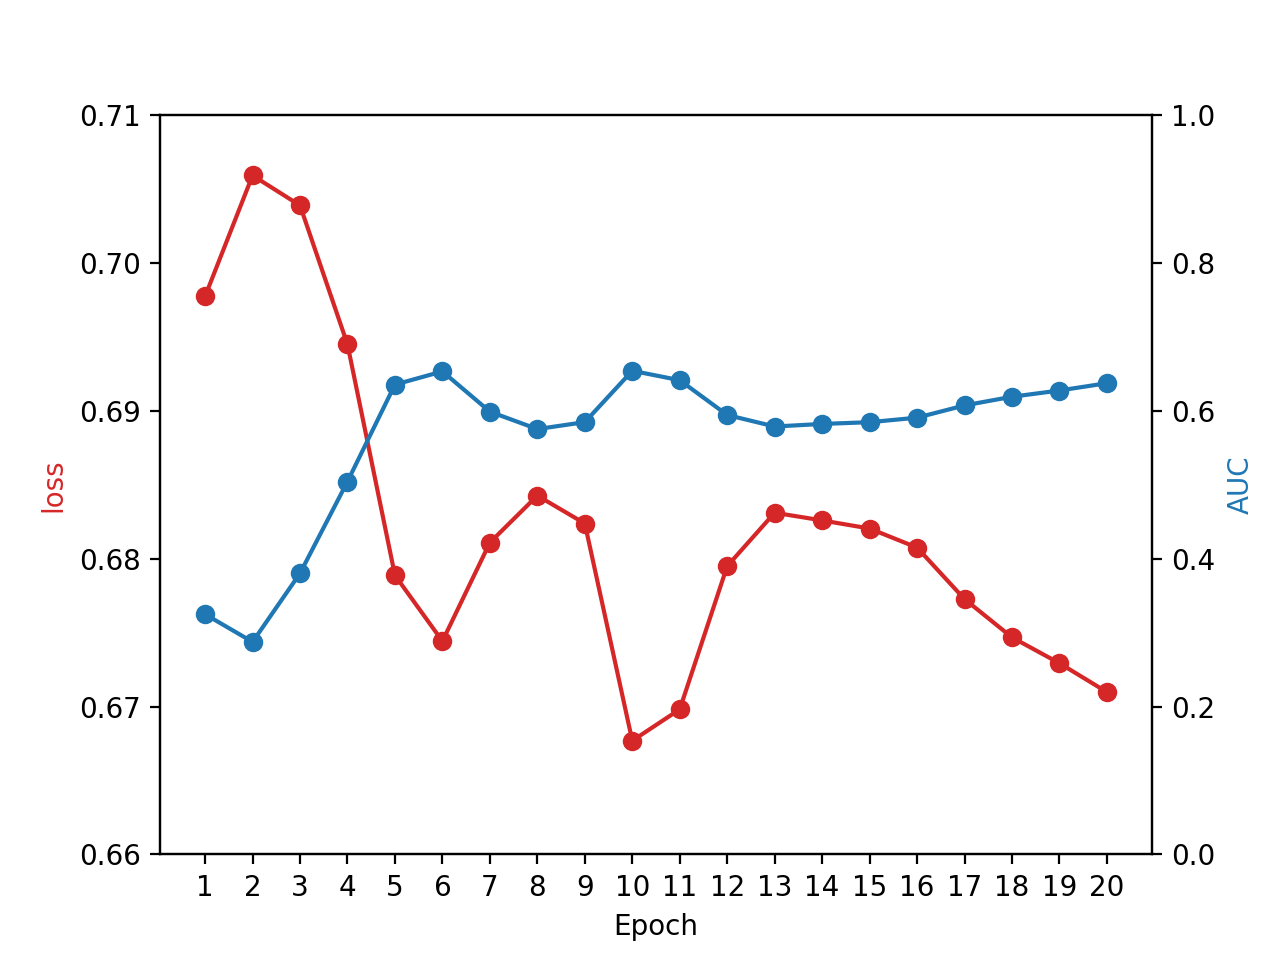
\includegraphics[width=\textwidth]{images/evaluation/Figure_18and19pureTrain.png}
         \caption{Train on window 19, 20, test on window 20}
         \label{fig:train_18_19_test_20}
     \end{subfigure}
    \caption{'Illustration of the impact of more or less adaptive incremental learning on the convergence behavior'.
    (left) No adaptive incremental learning: Training the model on window 1 and 2, then testing on window 20.
    (right) Full adaptive incremental learning: Training the model on window 18 and 19, then testing on window 20.}
    \label{fig:comparison_concept_drift}
\end{figure}

% 4. describe the results. Just tell us what are the most striking patterns
As epochs pass, we can see AUC score converges at a higher value which is above 0.6 in full incremental learning setup (i.e., training on window 18 and 19 which are more recent to the test window). As for the loss, the incremental setting is generally smaller than the non-incremental setting as well as converges at a much less significant value around 0.2.

% 5. discuss the results. Try to explain what we saw
The system with adaptive incremental learning outperforms the system without adaptive incremental learning regarding AUC score metric and cross-entropy loss, which verifies the impact of adaptive incremental learning on addressing concept drift.

\section{Importance-optimized learning with Guarantees}

Apart from adaptive learning, we seek to investigate how importance-optimized form of learning (that is, use output of Sketches instead of gt counts) affects the system in terms of classification performance when training on the same recent windows and testing on the same succeeding window.

% benchmark: all train on recent window: 16,17,18,19; same epochs
% compare Figure_16171819pure_epoch20.png and Figure_16pure_171819dirty.png

Our experiment will be conducted as follows. As benchmark for comparison purpose, we utilize fully-supervised learning, i.e., feed items with feature and ground truth labels to the model. We train on dataset of window 16, 17, 18, 19, then evaluate on window 20 at each epoch.
In the importance-optimized learning setup, we use semi-supervised learning: on window 16, we do the same as benchmark that is supervised training, but on subsequent windows 17, 18, 19, instead of feeding ground truth counts, we firstly apply count-min on those data to generate estimated counts, then we feed estimated counts as labels to the deep learning model for training. In the end, we evaluate on data from window 20 after each epoch of semi-supervised training.


In Figure~\ref{fig:comparison_dirty}, we demonstrate our observations.

\begin{figure}[htbp!]
     \centering
     \begin{subfigure}[b]{0.49\textwidth}
         \centering
         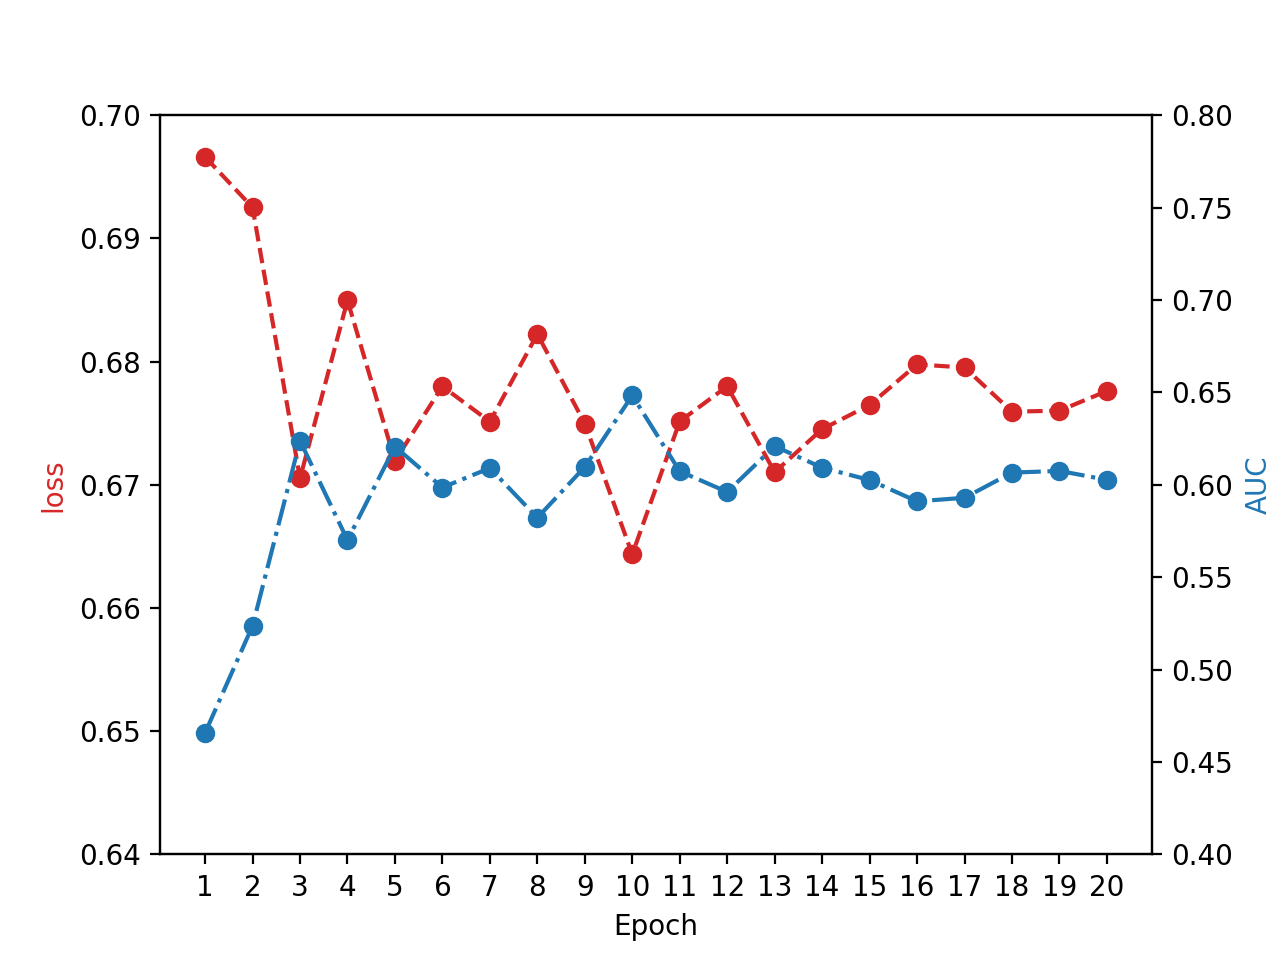
\includegraphics[width=\textwidth]{images/evaluation/Figure_16171819pure_epoch20.png}
         \caption{Pure Supervised learning}
         \label{fig:16171819pure}
     \end{subfigure}
     \hfill
     \begin{subfigure}[b]{0.49\textwidth}
         \centering
         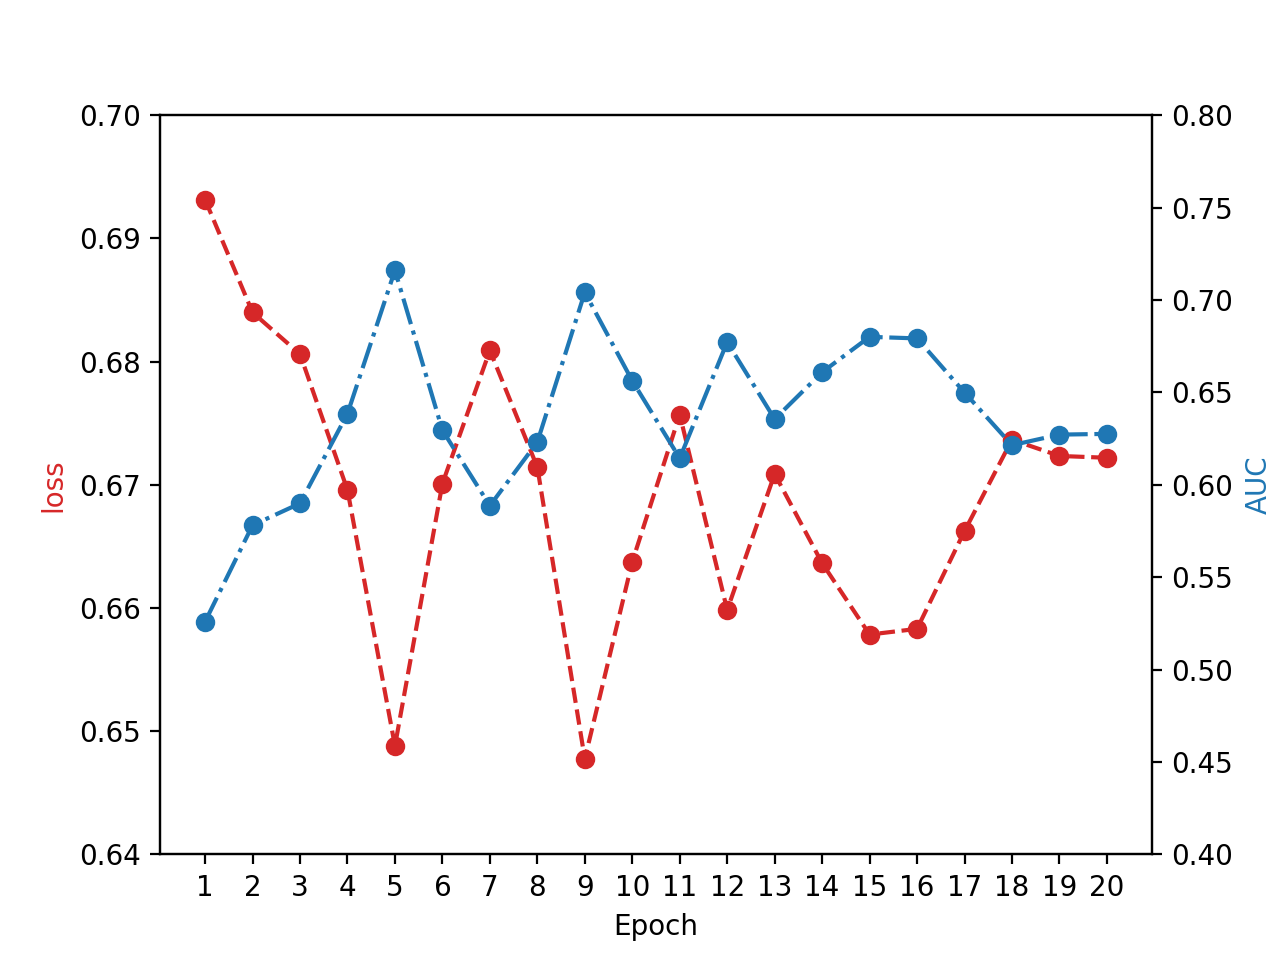
\includegraphics[width=\textwidth]{images/evaluation/Figure_16pure_171819dirty.png}
         \caption{Semi-supervised learning}
         \label{fig:16pure_171819dirty}
     \end{subfigure}
    \caption{Illustration showing gain of importance-optimized learning (right, pure train on window 16, relabel and semi-supervised train on window 17, 18, 19) compared to supervised-only learning (left, pure supervised-train on window 16, 17, 18, 19)}
    \label{fig:comparison_dirty}
\end{figure}

In the figure, we notice that the AUC metric in the setting of importance-optimized learning outperforms that in the setting of supervised-only learning at most epochs and also converge at a higher level. In addition, it reaches new high of our system at epoch 5 and 9, surpassing 0.7. 
The Loss value shows the similar effects. The semi-supervised setup stay mostly below supervised-only setup in terms of cross-entropy loss and converges at a lower value as well. 

Overall, with regard to classifying top and bottom items, the results confirm that our importance-optimized learning system is significantly better than the normal model trained with only ground truth counts. Considering the limited datasets we have, AUC scores over 0.7 are terrific and hence verify the power of importance-optimized learning.

\section{Top k Pyramid}

% 1. Say we want to investigate sth. and why it will bring us useful insights.
Gradual pooling to top-k is another big direction next to temporal continuity. We want to investigate how accurately the model can predict counts when adding top k pooling layers. We spend more resources on the items pooled (we pay more attention to them). That is, we try to obtain more semantically effective embeddings of these items.


% 2. Say how we investigate that thing, i.e., experimental setup.
We train the model with pooling setup on window 2 and 3, then test on windows 20 which is quite challenging because of the concept drift. For the batch size, we choose 1000. Thus, the model pools from 1000 to 500, from 500 to 200 and from 200 to 100 at last. We take mean squared error as loss function and mean absolute error as metrics so that we can emphasize on the regression performance.


\begin{figure}[htbp!]
	\centering
	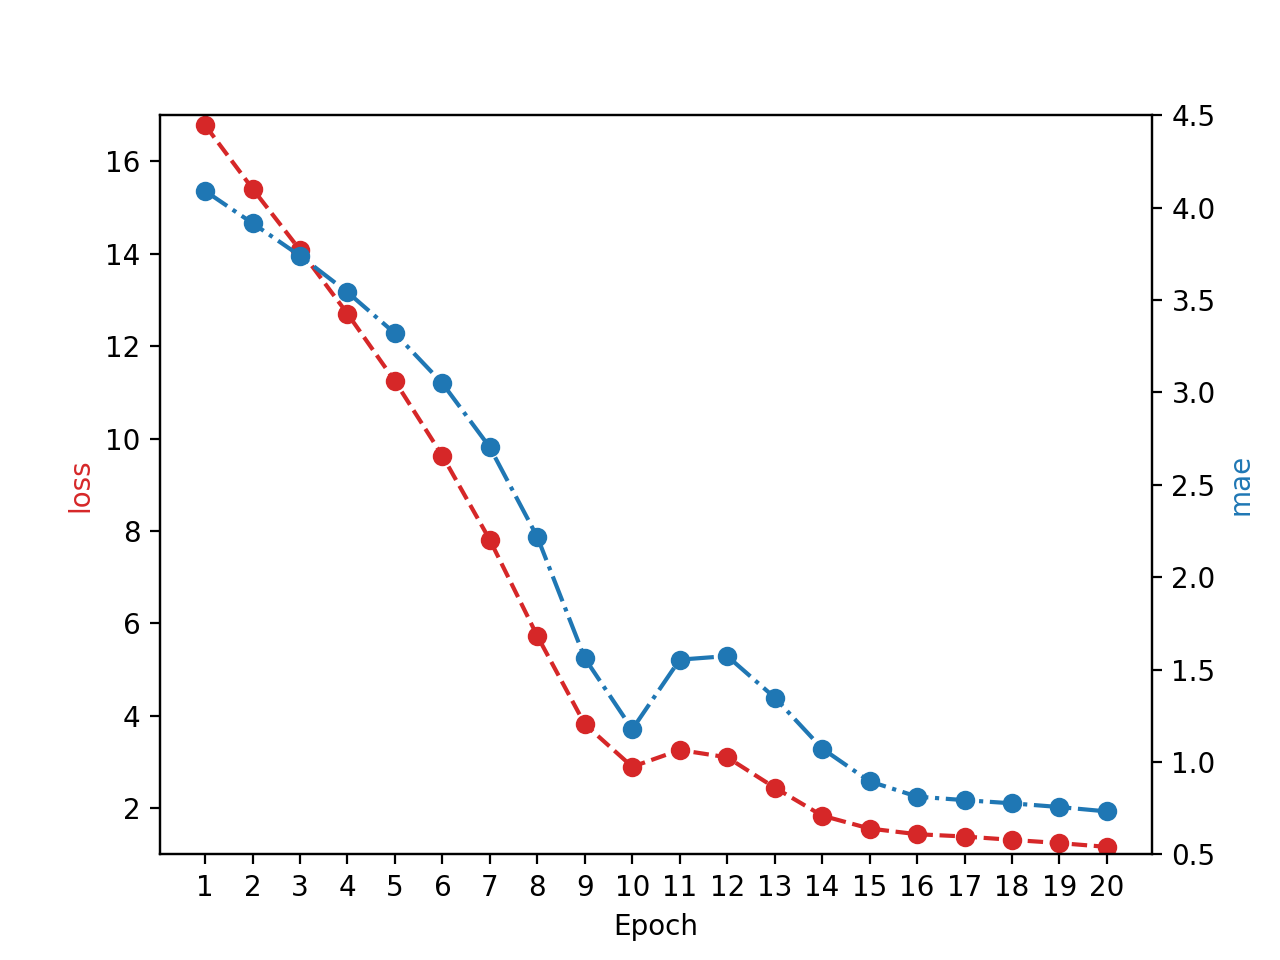
\includegraphics[width=0.6\linewidth]{images/plots/pyramid_performance.png}
	\caption{Count prediction performance of the top k pyramid model}
	\label{fig:pyramid_performance}
\end{figure}

% 3. Say our results are presented in Material XYZ (plot/table)
We illustrate our evaluations in figure~\ref{fig:pyramid_performance}.

% 4. describe the results. Just tell us what are the most striking patterns
According to the figure, we can see both of the MSE loss and the MAE metric dramatically go down when epoch goes from 1 to 20.

% 5. discuss the results. Try to explain what we saw
Considering the test data is fairly unfamiliar for the trained model, the obtained performance substantiates the validity of top k pyramid pooling. It is because our pyramid system is capable of characterizing the same information in a combination of more latent form on less-important elements and more explicit form on more-important elements.





























% Besides adaptive learning, the model performance can still be improved by applying an importance-optimized form of learning --use output of Sketches instead of gt counts. We belong to the tradition of \emph{Generative Adversarial Networks}~\cite{goodfellow2014generative} trying to zero out on the most relevant examples to learn on, but we go further by modeling importance in an explainable manner. We try to do about the same but with a prioritization not fully inferred but partially inferred in an optimized manner: with a selection inferred by the system itself to the best of its capacity, but values efficiently approximated with guarantees.

